\documentclass[11pt, aspectratio=169]{beamer}

\usetheme{metropolis}
\metroset{block=fill}

\usepackage[utf8]{inputenc}
\usepackage{amsmath, amssymb, physics}
\usepackage{tikz}
\usetikzlibrary{shapes.geometric, arrows.meta, positioning, fit, backgrounds, calc}
\usepackage{adjustbox}

\title{The Unitary Compiler Collection (UCC)}
\subtitle{Exact Classical Simulation via the Factored State Architecture}
\author{Unitary Foundation Team}
\date{\today}

\begin{document}

\maketitle

\begin{frame}{Agenda}
  \setbeamertemplate{section in toc}[sections numbered]
  \tableofcontents[hideallsubsections]
\end{frame}

% =======================================================
\section{The Simulation Bottleneck \& The Pivot}
% =======================================================

\begin{frame}{The Universal Simulation Bottleneck}
  Simulating fault-tolerant quantum circuits (FTQC) requires deep non-Clifford logic (e.g., $T$-gates). Standard exact simulators inevitably hit exponential walls:

  \vspace{0.5em}
  \begin{itemize}
      \item \textbf{Statevector Simulators (e.g., Qiskit):} Hit the \alert{$\mathcal{O}(2^N)$ Physical Memory Wall}. Cannot exceed $\sim$40-50 qubits regardless of circuit structure.
      \item \textbf{Stabilizer Rank (e.g., tsim):} Hit the \alert{$\mathcal{O}(2^{\alpha t})$ T-Count Wall}. Branches on every $T$-gate; times out on deep arithmetic logic.
      \item \textbf{Generalized Stabilizers (e.g., SOFT):} Avoids the T-count wall, but dynamic tableau pivoting across sparse vectors introduces heavy \alert{$\mathcal{O}(n^2)$ overhead per shot}.
  \end{itemize}
\end{frame}

\begin{frame}{Motivating Example: Magic State Cultivation (MSC)}
  \textbf{The Goal:} Evaluate Magic State Cultivation protocols over $10^{12}$ shots to escape the physical noise floor.

  \vspace{1em}
  \begin{alertblock}{The Challenge}
      \begin{itemize}
          \item Highly probabilistic (requires fast-fail post-selection).
          \item Deep non-Clifford $T$-gate entanglement.
          \item Standard tools simply cannot scale to trillions of shots at FTQC hardware scales without massive GPU clusters.
      \end{itemize}
  \end{alertblock}
\end{frame}

\begin{frame}{The ``New'' UCC: A Strategic Pivot}
  \textbf{Previous UCC:} An open-source routing and bridging compiler. \\
  \textbf{New UCC:} A \textbf{Multi-Level Compiler} and \textbf{Schrödinger Virtual Machine (SVM)} built explicitly for the Early FTQC Era.

  \vspace{1em}
  \begin{itemize}
      \item We break the exponential bottlenecks by decoupling deterministic routing from probabilistic non-Clifford entanglement.
      \item UCC scales exponentially \textit{only} with the \textbf{Peak Active Rank} ($k_{\max}$).
  \end{itemize}
\end{frame}

% =======================================================
\section{The Core Theory: The Factored State}
% =======================================================

\begin{frame}{Circuit Composition \& The Heisenberg Mapping}
  We partition all quantum operations into two sets:
  \begin{enumerate}
      \item \textbf{Deterministic:} Clifford Unitaries ($C \in \mathcal{C}_n$).
      \item \textbf{Active:} Non-Clifford rotations ($T$), Measurements, Pauli Noise.
  \end{enumerate}

  \vspace{1em}
  Instead of applying Cliffords to the statevector, we map Active operations \textit{backward} through the Clifford frame ($U_C$) into a static virtual basis:
  \begin{equation*}
      \tilde{P}_O = (U_C^{(t)})^\dagger P_O U_C^{(t)}
  \end{equation*}

  \textit{Insight:} Coordinate mapping is defined entirely by Pauli tracking, completely independent of complex amplitudes!
\end{frame}

\begin{frame}{The Factored State Equation}
  We define the exact physical quantum state at time $t$ via a strict factorization:
  \begin{equation*}
      \Large |\psi^{(t)}\rangle = \gamma^{(t)} U_C^{(t)} \tilde{P}^{(t)} \Big( |\phi^{(t)}\rangle_A \otimes |0\rangle_D \Big)
  \end{equation*}

  \vspace{0.2em}
  \begin{itemize}
      \item \textbf{$U_C^{(t)}$ (Clifford Frame):} Deterministic geometric coordinate mapping.
      \item \textbf{$\tilde{P}^{(t)}$ (Virtual Pauli Frame):} Tracks discrete stochastic errors via virtual $X$ and $Z$ vectors: $\tilde{P}^{(t)} = \bigotimes_{j=0}^{n-1} X_j^{x_j^{(t)}} Z_j^{z_j^{(t)}}$. Evaluated via $\mathcal{O}(1)$ bitwise XORs.
      \item \textbf{$|\phi^{(t)}\rangle_A$ (Active Statevector):} A dense $2^k$ array tracking non-Clifford superposition on $k$ \textit{Active} virtual qubits.
      \item \textbf{$|0\rangle_D$ (Dormant Qubits):} The $n-k$ qubits mathematically locked in $|0\rangle$.
      \item \textbf{$\gamma^{(t)}$ (Global Scalar):} Tracks continuous phases and deferred normalization.
  \end{itemize}
\end{frame}

\begin{frame}{Virtual Compression (The ``Secret Sauce'')}
  How do we apply a mapped multi-qubit operator (e.g., $\tilde{P} = X_0 \otimes Z_1$) without evaluating a full $2^n$ statevector?

  \vspace{0.5em}
  \begin{block}{Lemma 2: Exact Pauli Compression}
      The Multi-Level compiler constructively synthesizes a sequence of virtual Cliffords $V$ to compress \textit{any} multi-qubit Pauli onto a \textbf{single virtual axis} $v$. ($V \tilde{P} V^\dagger = P_v$).
  \end{block}

  \begin{block}{Lemma 1: Zero-Cost Dormancy}
      If $V$ uses a Dormant qubit as a control (e.g., CNOT$_{D \to A}$), it mathematically acts as the Identity on the Active statevector. \textbf{Zero FLOPs required.}
  \end{block}
\end{frame}

\begin{frame}{Applying the Compression: Where does $V$ go?}
  If we apply virtual Cliffords $V$ to compress an operator $O(\tilde{P})$, how is the global state preserved?

  \vspace{0.5em}
  The compiler mathematically inserts the identity $V^\dagger V = I$ into the factored state, effectively \textbf{pushing it forward}:
  \begin{equation*}
      \dots \underbrace{U_C^{(t)} \alert{V^\dagger}}_{\text{1. Offline Frame}} \;\; \underbrace{\Big[ \alert{V} O(\tilde{P}) \alert{V^\dagger} \Big]}_{\text{2. Localized Op}} \;\; \underbrace{\Big( \alert{V} \tilde{P}^{(t)} \alert{V^\dagger} \Big)}_{\text{3. Pauli Tracker}} \;\; \underbrace{\alert{V} \Big( |\phi^{(t)}\rangle_A \otimes |0\rangle_D \Big)}_{\text{4. Active Array}}
  \end{equation*}

  \vspace{1em}
  The transformation $V$ distributes exactly where it is needed:
  \begin{enumerate}
      \item \textbf{Clifford Frame:} Absorbs the inverse offline ($U_C \leftarrow U_C V^\dagger$).
      \item \textbf{The Operation:} Compresses to act on a single virtual axis ($O(P_v)$).
      \item \textbf{Pauli Frame:} Is dynamically conjugated via $\mathcal{O}(1)$ bitwise XORs.
      \item \textbf{Active Array:} Undergoes the transformation $V$ (which costs \textbf{zero FLOPs} if controlled by a dormant qubit!).
  \end{enumerate}
\end{frame}

% =======================================================
\section{Walkthrough: A Toy Example}
% =======================================================

\begin{frame}{Walkthrough: Step-by-Step Factored State}
  \begin{columns}[T]
    \begin{column}{0.4\textwidth}
      \textbf{Circuit} (2 Qubits)
      \vspace{0.5em}

      \only<1>{$\rightarrow$ Init $|00\rangle$\\ \color{gray} Phys $H(q_0)$\\ \color{gray} Phys $T(q_0)$\\ \color{gray} Phys CX$(q_0 \to q_1)$\\ \color{gray} Measure $q_1$}
      \only<2>{\color{gray} Init $|00\rangle$\\ \color{black}$\rightarrow$ Phys $H(q_0)$\\ \color{gray} Phys $T(q_0)$\\ \color{gray} Phys CX$(q_0 \to q_1)$\\ \color{gray} Measure $q_1$}
      \only<3>{\color{gray} Init $|00\rangle$\\ \color{gray} Phys $H(q_0)$\\ \color{black}$\rightarrow$ Phys $T(q_0)$ \textit{(Compile)}\\ \color{gray} Phys CX$(q_0 \to q_1)$\\ \color{gray} Measure $q_1$}
      \only<4>{\color{gray} Init $|00\rangle$\\ \color{gray} Phys $H(q_0)$\\ \color{black}$\rightarrow$ Phys $T(q_0)$ \textit{(Execute)}\\ \color{gray} Phys CX$(q_0 \to q_1)$\\ \color{gray} Measure $q_1$}
      \only<5>{\color{gray} Init $|00\rangle$\\ \color{gray} Phys $H(q_0)$\\ \color{gray} Phys $T(q_0)$\\ \color{black}$\rightarrow$ Phys CX$(q_0 \to q_1)$\\ \color{gray} Measure $q_1$}
      \only<6>{\color{gray} Init $|00\rangle$\\ \color{gray} Phys $H(q_0)$\\ \color{gray} Phys $T(q_0)$\\ \color{gray} Phys CX$(q_0 \to q_1)$\\ \color{black}$\rightarrow$ Measure $q_1$}

      \vspace{1.5em}
      \only<3>{\textit{\footnotesize \textbf{Why no $I/Z$ branching?}\\ $T \propto \exp(-i \frac{\pi}{8} Z)$. Because $I$ is invariant, $V$ distributes directly into the exponent: $\exp(-i\frac{\pi}{8} \alert{V Z_0 V^\dagger})$.}}
      \only<5>{\alert{\textbf{Key Insight:}}\\ \footnotesize The physical CX entangles the qubits, but because it is a Clifford, the Active Array doesn't care! It costs zero FLOPs.}
    \end{column}

    \begin{column}{0.6\textwidth}
      \begin{block}{System State at $t$}
        \only<1>{
          $U_C = I$, \quad $\tilde{P}^{(t)} = I$ \\
          $A = \emptyset, \quad D = \{0, 1\} \quad \mathbf{(k=0)}$ \\
          $|\phi\rangle_A = [1], \quad \gamma = 1.0$
        }
        \only<2>{
          \textbf{Action:} Update deterministic frame offline.\\
          \vspace{0.5em}
          $U_C = H_0$ \\
          $\tilde{P}^{(t)} = I$ \\
          $A = \emptyset, \quad D = \{0, 1\} \quad \mathbf{(k=0)}$ \\
          $|\phi\rangle_A = [1]$ \quad \alert{\textit{(Zero FLOPs!)}}
        }
        \only<3>{
          \textbf{Compile T-Gate (Rotation about Z):}\\
          $T \propto \exp(-i \frac{\pi}{8} \mathbf{Z_0})$. We track the generator!\\
          \vspace{0.5em}
          \textit{We don't branch into $I$ and $Z$ universes!} Physical $Z_0$ maps through $U_C$ to virtual \alert{$\mathbf{X_0}$}.\\
          \vspace{0.5em}
          Compiler applies $V = H_0$ to align $X_0 \to Z_0$ for the continuous diagonal phase.
        }
        \only<4>{
          \textbf{Execute T-Gate (Dimensionality Expansion):}\\
          \vspace{0.5em}
          Virtual $V^\dagger$ pushes into $U_C$ ($U_C \leftarrow U_C \cdot H_0 = I$).\\
          Axis $q_0$ activates.\\
          $A = \{0\}, \quad D = \{1\} \quad \mathbf{(k=1)}$ \\
          $|\phi\rangle_A = [1, e^{i\pi/4}]^T$ \quad \textit{(Array Doubles!)} \\
          $\gamma = e^{i\pi/8} / \sqrt{2}$ \quad \textit{(Absorbs global phase)}
        }
        \only<5>{
          \textbf{Physical Entanglement:}\\
          Clifford gate maps directly into the offline frame.\\
          \vspace{0.5em}
          $U_C \leftarrow \text{CX}_{0\to 1} \cdot U_C = \text{CX}_{0\to 1}$ \\
          $A = \{0\}, \quad D = \{1\} \quad \mathbf{(k=1)}$ \\
          $|\phi\rangle_A = [1, e^{i\pi/4}]^T$ \\
          \vspace{0.5em}
          \alert{\textit{The array is completely untouched!}}
        }
        \only<6>{
          \textbf{Action:} Projective Measurement. Outcome $m$.\\
          Physical $Z_1$ pushes through $\text{CX}_{0\to 1}$ to \alert{$\mathbf{Z_0 \otimes Z_1}$}.\\
          \vspace{0.5em}
          Virtual $V = \text{CX}_{1 \to 0}$ compresses it to $Z_0$. Measure Active $q_0$.\\
          $\tilde{P}^{(t)} \leftarrow$ Updates $\mathbf{x}, \mathbf{z}$ tracking. \\
          $A = \emptyset, \quad D = \{0, 1\} \quad \mathbf{(k=0)}$ \\
          $|\phi\rangle_A = [1]$ \quad \textit{(Array Halves!)} \\
          $\gamma \leftarrow \gamma / \sqrt{p_m}$
        }
      \end{block}
    \end{column}
  \end{columns}
\end{frame}

% =======================================================
\section{Software Architecture}
% =======================================================

\begin{frame}{The ``Aha!'' Moment: Theorem 1}
  Look closely at the walkthrough. When did $U_C$ update? When did the Pauli operators compress?

  \vspace{1em}
  \begin{alertblock}{Theorem 1: Clifford Frame Determinism}
      The evolution of the Clifford Frame $U_C$ and the dimensional bounds of the active set ($k_{\max}$) depend \textit{exclusively} on the sequence of physical operations. They are strictly independent of probabilistic measurement outcomes or continuous non-Clifford amplitudes.
  \end{alertblock}

  \vspace{1em}
  \textbf{Consequence:} We do not need to do heavy tableau math online. We cleanly split the simulation into an \textbf{Offline Multi-Level Compiler} and an \textbf{Online Virtual Machine}.
\end{frame}

\begin{frame}{Decoupling Computational Complexity}
  \textbf{1. Multi-Level Compiler (Offline):}
  \begin{itemize}
      \item Eats the $\mathcal{O}(G n^2)$ topological matrix tracking.
      \item Evaluates optimal Pauli Compressions to single virtual axes.
      \item Computes global algebraic optimizations over the timeless \textbf{Heisenberg IR (HIR)}.
  \end{itemize}

  \vspace{1em}
  \textbf{2. The Schrödinger Virtual Machine (Online):}
  \begin{itemize}
      \item Executes in strictly bounded $\mathcal{O}(2^{k_{\max}})$.
      \item No dynamic memory allocation. Executes purely localized RISC bytecode.
      \item \textit{Note: The extreme C++ engineering making the VM fast (32-byte opcodes, branchless hardware popcounts) is a topic for a future deep-dive!}
  \end{itemize}
\end{frame}

\begin{frame}{UCC Architecture Diagram}
  \begin{center}
    \adjustbox{max width=0.95\textwidth, max height=0.85\textheight}{
      \begin{tikzpicture}[
        >=Stealth,
        font=\sffamily,
        node distance=1.2cm and 2.0cm,
        impl/.style={rectangle, draw=blue!80!black, fill=blue!5, thick, minimum width=5.5cm, minimum height=1.6cm, align=center, rounded corners=1ex, font=\large\bfseries},
        impl-io/.style={rectangle, draw=black!80, fill=gray!10, thick, minimum width=3.5cm, minimum height=1.0cm, align=center, rounded corners=1ex, font=\normalsize\bfseries},
        fut/.style={rectangle, draw=gray!50, fill=white, dashed, thick, minimum width=5.5cm, minimum height=1.6cm, align=center, rounded corners=1ex, font=\normalsize, text=gray!80!black},
        fut-io/.style={rectangle, draw=gray!50, fill=white, dashed, thick, minimum width=3.5cm, minimum height=1.0cm, align=center, rounded corners=1ex, font=\normalsize, text=gray!80!black},
        arr-impl/.style={->, line width=0.6mm, draw=blue!80!black},
        arr-fut/.style={->, line width=0.6mm, dashed, draw=gray!50}
      ]

      % Top Row (Left to Right)
      \node[impl-io] (in-stim) {Extended Stim\\ \small (Native Format)};
      \node[fut-io, above=0.2cm of in-stim] (in-qasm) {OpenQASM 3};
      \node[fut-io, below=0.2cm of in-stim] (in-qiskit) {Qiskit / Cirq};

      \node[impl, right=2cm of in-stim] (fe) {Front-End Compiler\\ \normalsize Physical Rewinding \&\\ \normalsize Clifford Absorption};

      % Middle Row (Right to Left)
      \node[impl, below=1.5cm of fe] (me) {Middle-End Optimizer\\ \normalsize Global Commutation \&\\ \normalsize Algebraic Fusion (HIR)};

      \node[impl, left=2cm of me] (be) {Compiler Back-End\\ \normalsize Virtual Compression \&\\ \normalsize RISC Bytecode Emission};

      % Bottom Row
      \node[impl, below=1.5cm of be] (vm) {Schrödinger VM\\ \normalsize $\mathcal{O}(2^k)$ Execution over\\ \normalsize Contiguous Array};

      \node[fut, below=1.5cm of me] (hw) {Hardware Routers\\ \normalsize (e.g., tqec / NISQ)};

      \node[impl-io, below=0.8cm of vm] (out-bits) {Sampled Bitstrings};

      % Arrows
      \draw[arr-impl] (in-stim.east) -- (fe.west);
      \draw[arr-fut] (in-qasm.east) to[out=0, in=150] (fe.150);
      \draw[arr-fut] (in-qiskit.east) to[out=0, in=210] (fe.210);

      \draw[arr-impl] (fe.south) -- node[right, font=\normalsize\bfseries] {Heisenberg IR} (me.north);
      \draw[arr-impl] (me.west) -- node[above, font=\normalsize\bfseries] {Optimized HIR} (be.east);

      \draw[arr-impl] (be.south) -- node[right, font=\normalsize\bfseries] {RISC Bytecode} (vm.north);
      \draw[arr-impl] (vm.south) -- (out-bits.north);

      \draw[arr-fut] (me.south) -- node[right, font=\normalsize] {Opt. HIR} (hw.north);

      % Legend
      \node[rectangle, draw=gray!50, fill=gray!5, rounded corners=0.5ex, thick, inner sep=6pt, below=0.8cm of hw] (legend) {
          \begin{tikzpicture}
              \draw[blue!80!black, fill=blue!5, thick, rounded corners=0.2ex] (0,0) rectangle (0.6, 0.3);
              \node[anchor=west, font=\normalsize\bfseries, text=black, inner sep=4pt] at (0.6, 0.15) {UCC Implemented};
              \draw[gray!50, fill=white, dashed, thick, rounded corners=0.2ex] (4.5,0) rectangle (5.1, 0.3);
              \node[anchor=west, font=\normalsize, text=gray!80!black, inner sep=4pt] at (5.1, 0.15) {Future / Ecosystem};
          \end{tikzpicture}
      };

      \end{tikzpicture}
    }
  \end{center}
\end{frame}

% =======================================================
\section{Benchmarks \& Results}
% =======================================================

\begin{frame}[standout]
  Live Demo \\ \normalsize \textit{Manually driving compiler and evaluating active bounds}
\end{frame}

\begin{frame}{The ``Three Walls'' Benchmark}
  Each circuit has $N$ physical qubits, $k$ peak active non-Clifford virtual qubits, and $t$ total $T$-gates. We isolate each axis on identical random Clifford+$T$ circuits, comparing UCC against Qiskit-Aer (statevector) on a single CPU core:

  \vspace{0.3em}
  \begin{itemize}
      \item \textbf{Panel A --- Physical Qubit Wall ($N$):} Fix $k{=}12$, $t{=}20$, sweep $N$. Qiskit scales as $\mathcal{O}(2^N)$; it times out at $N{=}28$ and OOMs at $N{=}29$. \alert{UCC remains flat at $\sim$60\,ms.}
      \item \textbf{Panel B --- Active Rank Wall ($k$):} Fix $N{=}24$, $t{=}40$, sweep $k$. Qiskit is constant (always pays $2^{24}$). \alert{UCC scales as $\mathcal{O}(2^k)$}, revealing its honest exponential bound.
      \item \textbf{Panel C --- Gate Depth Wall ($t$):} Fix $N{=}26$, $k{=}12$, sweep $t$. Both simulators scale linearly in $t$. \textit{Planned:} adding \texttt{tsim} (stabilizer-rank) to Panel~C will expose the $\mathcal{O}(2^{\alpha t})$ wall that UCC avoids.
  \end{itemize}
\end{frame}

\begin{frame}{Three Walls: UCC vs.\ Qiskit-Aer}
  \begin{center}
    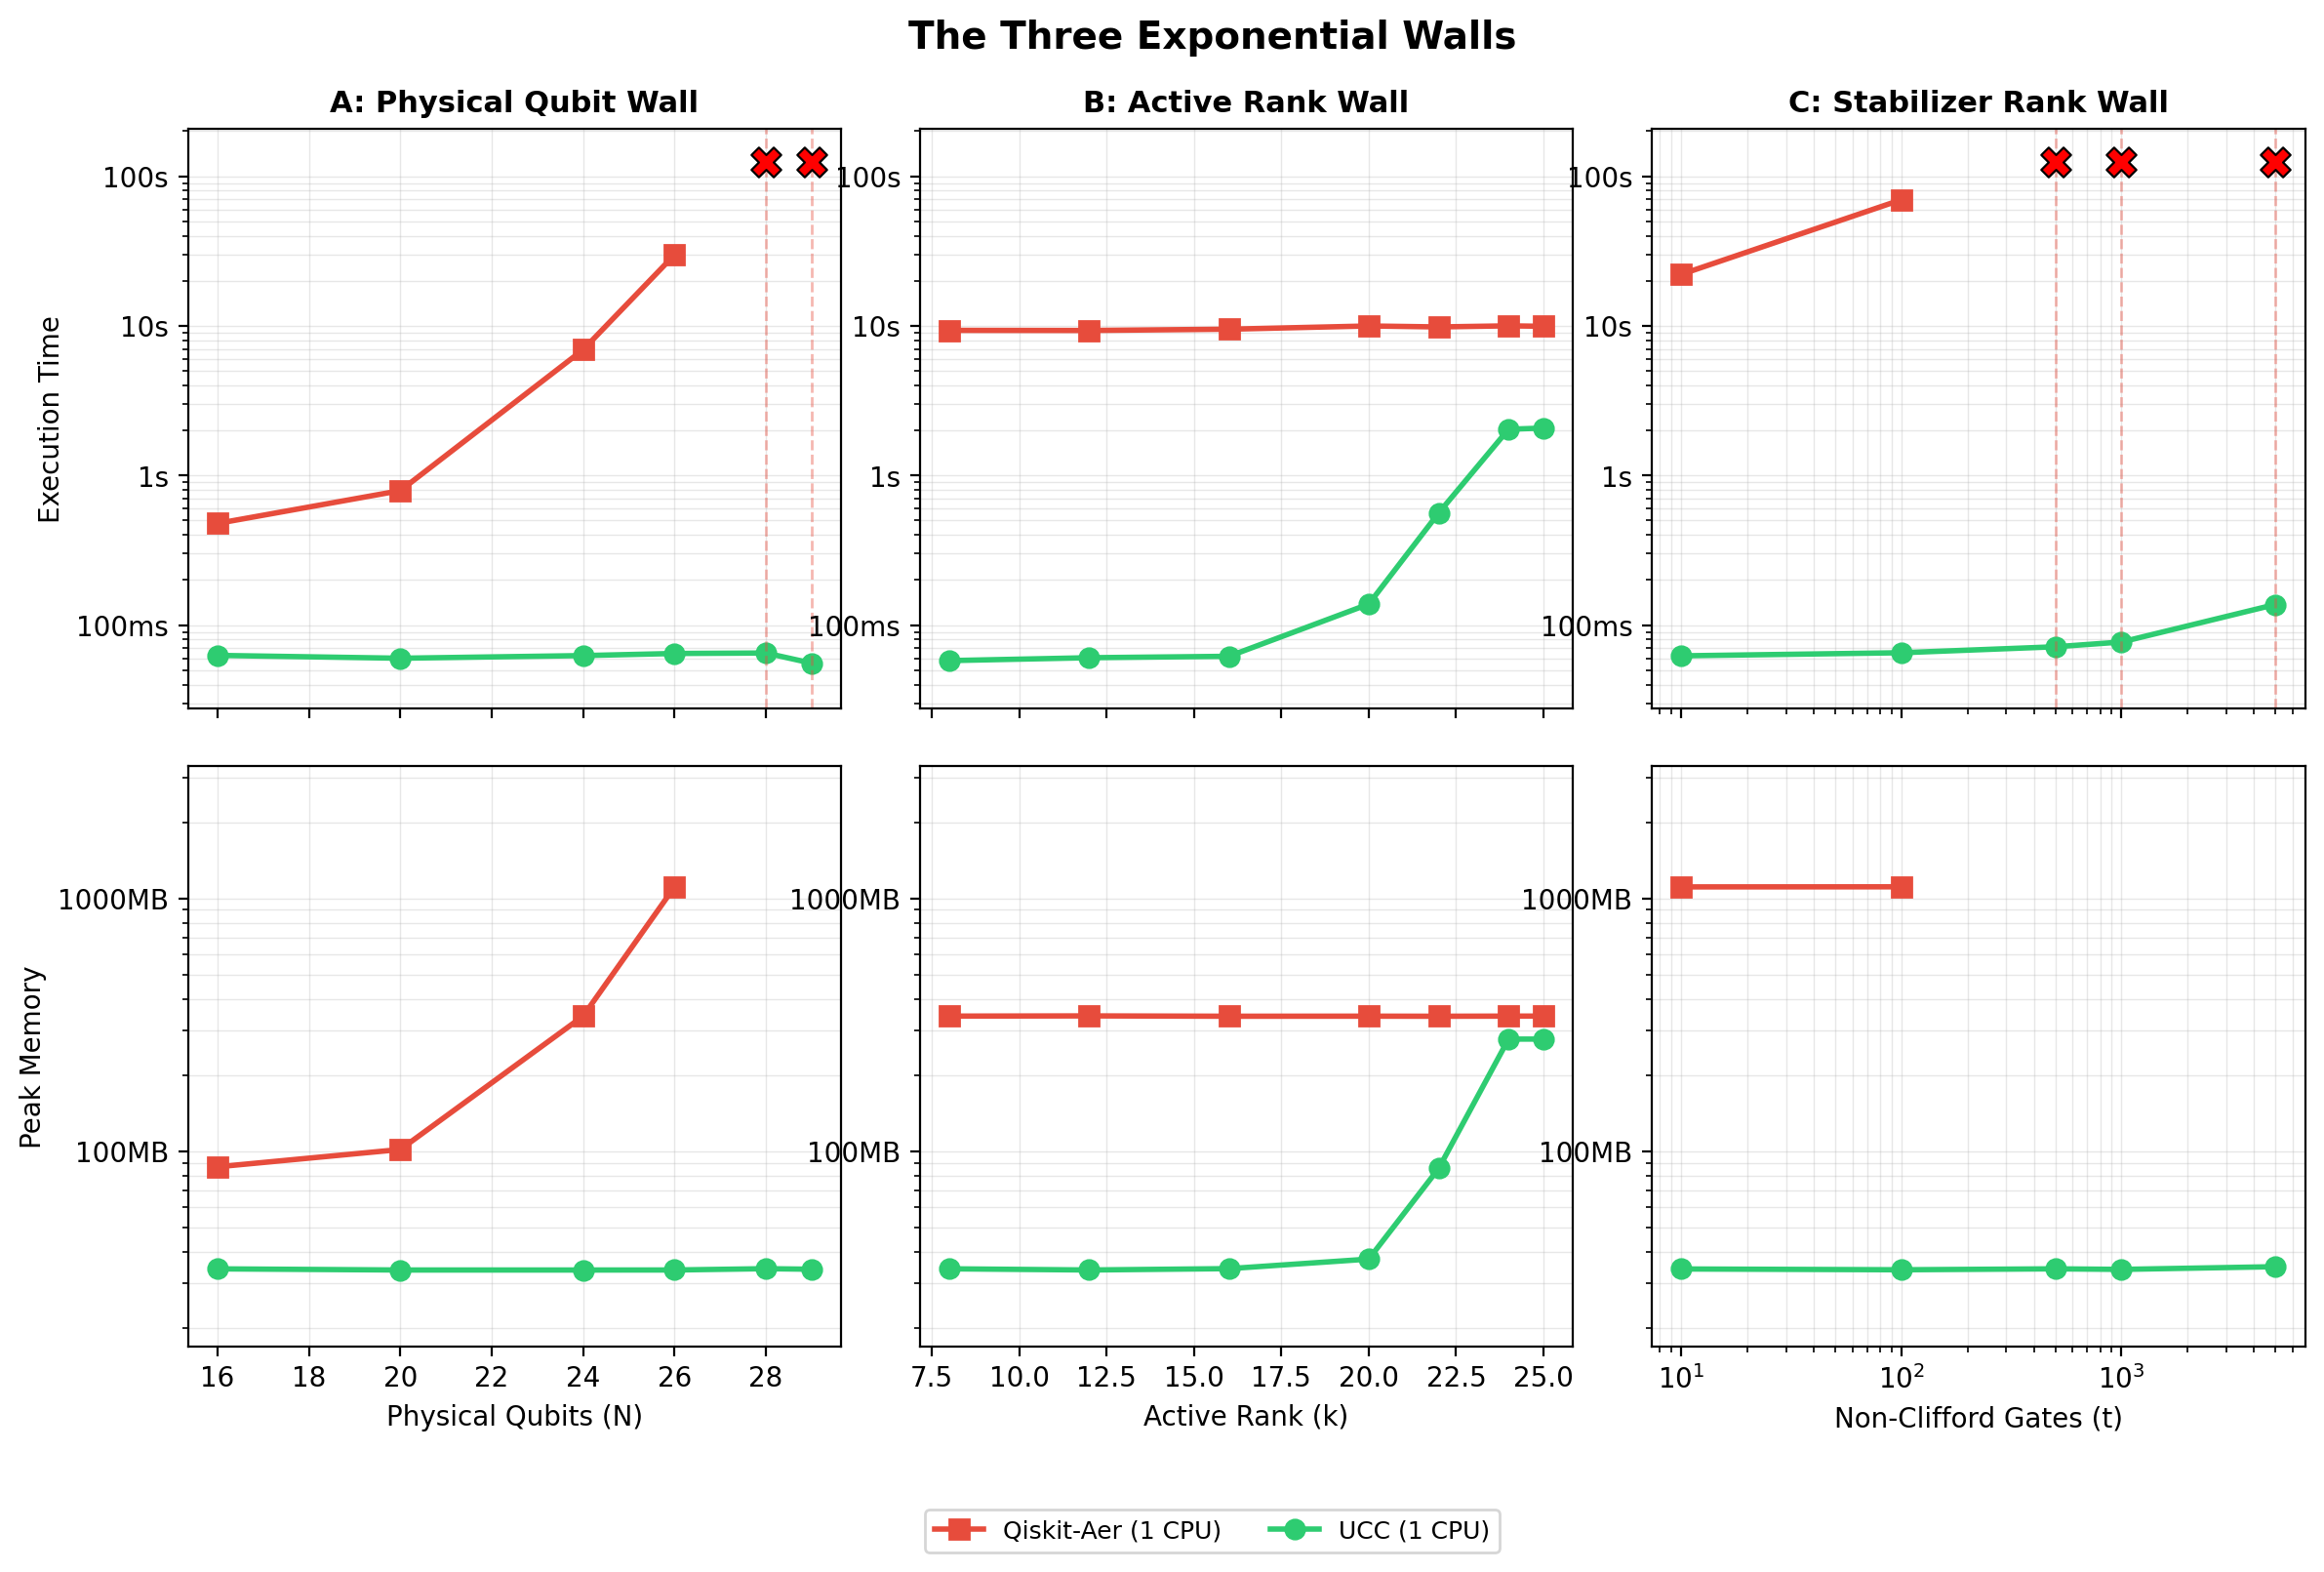
\includegraphics[width=\textwidth, height=0.82\textheight, keepaspectratio]{three_walls.png}
  \end{center}
  \vspace{-0.5em}
  {\scriptsize Dashed/{\color{red}\Large$\times$} = timeout (120\,s) / OOM (6.5\,GB). Single-threaded, Intel Xeon 8259CL, 7.2\,GB RAM.}
\end{frame}

\begin{frame}{Scaling Up: Magic State Cultivation}
  \textbf{Goal:} Evaluate Magic State Cultivation (MSC) protocols at scale.

  \vspace{1em}
  \textbf{Phase 1 Validated ($d=5$ Cultivation Step):}
  \begin{itemize}
      \item The SOFT simulator (Li et al. 2025) previously required a 16-GPU cluster to process online dynamic tableaus for this 42-qubit circuit.
      \item By utilizing \textit{Dense Survivor Sampling} and fast-fail opcodes, \textbf{UCC accurately matched the results on a single physical CPU core}.
      \item \textbf{Estimated Trillion-Shot Cost:} $\sim$\$500 and 29 hours on an AWS spot cluster to fully map this specific $d=5$ protocol curve.
  \end{itemize}

  \vspace{0.5em}
  \textbf{Next Target:} We are actively estimating the runtime and cost required to execute the \textit{full} 463-qubit ($d=7$) end-to-end cultivation protocol.
\end{frame}

% =======================================================
\section{Next Steps \& Discussion}
% =======================================================

\begin{frame}{Feedback \& Discussion}
  \begin{enumerate}
      \item \textbf{Project Scope:} Should this Multi-Level VM architecture fully replace the old UCC (bridging/routing), or sit alongside it as a specialized engine?
      \vspace{1em}
      \item \textbf{Publication Strategy:} What are the most critical benchmarks to include in the initial paper? (e.g., 3-Walls, FastTODD optimization, MSC validation).
      \vspace{1em}
      \item \textbf{Narrative Framing:} Does positioning UCC as ``A Multi-Level Compiler \& Execution Engine for the Early Fault Tolerance Era'' resonate with the foundation's vision?
  \end{enumerate}
\end{frame}

\begin{frame}[standout]
  Thank You! \\
  \vspace{0.5cm}
  \normalsize Questions?
\end{frame}

\end{document}
